\section{Problem (5)}
	The figure shows three forces applied to a trunk that moves leftward by $2.3 \ m$ over a frictionless floor. The force magnitudes are $F_{1} = 5.3 \ N$, $F_{2} = 6.7 \ N$, and $F_{3} = 4.1 \ N$ and the indicated angle is $\theta = 69^{o}$. During the displacement, what is the net work done on the trunk by the three forces?

	\begin{figure}[H]
		\begin{center}
			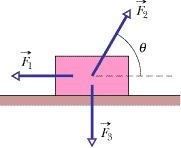
\includegraphics[scale=1]{hw7_problem5}
			\caption{Illustration of Problem 5}
			\label{fig:hw7_problem5}
		\end{center}
	\end{figure}

	\textbf{R:}

	\begin{align}
		W_{1} = \ &F_{1}r \cos \theta_{1}& \notag \\
		= \ &(5.3 \ N)(2.3 \ m) \cos 0^{o}& \notag \\
		= \ &12.19 \ N \times m = 12.19 J& \notag \\
		W_{2} = \ &F_{2}r \cos \theta_{2}& \notag \\
		= \ &(6.7 \ N)(2.3 \ m) \cos 111^{o}& \notag \\
		= \ &-5.52 \ N \times m = -5.52 \ J& \notag \\
		W_{3} = \ &F_{3}r \cos \theta_{3}& \notag \\
		= \ &(4.1 \ N)(2.3 \ m) \cos 90^{o}& \notag \\
		= \ &0& \notag \\
		W_{net} = \ &W_{1} + W_{2} + W_{3}& \notag \\
		= \ &(12.19 \ J) + (-5.52 \ J) + (0)& \notag \\
		= \ &6.67 \ J&
	\end{align}
